\section{Progettazione logica}
Una volta aver ristrutturato lo schema concettuale mostrato in Figura \ref{uml:schema_concettuale} si procede traducendo le varie associazioni descritte in Figura \ref{uml:schema_ristrutturato}. Iniziamo col tradurre direttamente tutte le classi. Man mano che si andranno a tradurre le varie associazioni andremo a modificare la struttura dei vari schemi relazionali laddove necessario.
\subsection{Traduzione delle classi}
Si ha quindi:

	\begin{tabular}{|l|l|l|}
		\multicolumn{3}{l}{\textsc{Ente}}\\ \hline
		\underline{id\_ente} & nome & sigla \\ \hline
	\end{tabular}


	\begin{tabular}{|l|l|l|l|l|l|}
		\multicolumn{6}{l}{\textsc{Sede}} \\ \hline
		\underline{id\_sede} & nome & via & civico & cap & city \\ \hline
	\end{tabular}


	\begin{tabular}{|l|l|}
		\multicolumn{2}{l}{\textsc{Sponsor}} \\ \hline
		\underline{id\_Sponsor} & Nome \\ \hline
	\end{tabular}


	\begin{tabular}{|l|l|}
		\multicolumn{2}{l}{\textsc{Comitato}} \\ \hline
		\underline{id\_Comitato} & Tipologia \\ \hline
	\end{tabular}


	\begin{tabular}{|l|l|l|l|l|}
		\multicolumn{5}{l}{\textsc{Organizzatore}} \\ \hline
		\underline{id\_Organizzatore} & Nome & Cognome & Titolo & Email \\ \hline
	\end{tabular}


	\begin{tabular}{|l|l|l|}
		\multicolumn{3}{l}{\textsc{Sala}} \\ \hline
		\underline{id\_Sala} & Nome & Capienza \\ \hline
	\end{tabular}


	\begin{tabular}{|l|l|l|l|l|}
		\multicolumn{5}{l}{\textsc{Conferenza}} \\ \hline
		\underline{id\_Conferenza} & Nome & Descrizione & Inizio & Fine \\ \hline
	\end{tabular}


	\begin{tabular}{|l|l|l|l|l|}
		\multicolumn{5}{l}{\textsc{Partecipante}} \\ \hline
		\underline{id\_Partecipante} & Nome & Cognome & Titolo & Email \\ \hline
	\end{tabular}


	\begin{tabular}{|l|l|l|l|}
		\multicolumn{4}{l}{\textsc{Sessione}} \\ \hline
		\underline{id\_Sessione} & Nome & Inizio & Fine \\ \hline
	\end{tabular}


	\begin{tabular}{|l|l|l|}
		\multicolumn{3}{l}{\textsc{Valuta}} \\ \hline
		\underline{Iso} & Nome & Simbolo \\ \hline
	\end{tabular}


	\begin{tabular}{|l|l|l|l|l|}
		\multicolumn{5}{l}{\textsc{Speaker}} \\ \hline
		\underline{id\_Speaker} & Nome & Cognome & Titolo & Email \\ \hline
	\end{tabular}


	\begin{tabular}{|l|}
		\multicolumn{1}{l}{\textsc{Programma}} \\ \hline
		\underline{Id\_Programma} \\ \hline
	\end{tabular}


	\begin{tabular}{|l|l|l|l|}
		\multicolumn{4}{l}{\textsc{Intervallo}} \\ \hline
		\underline{id\_Intervallo} & Tipologia & Inizio & Fine \\ \hline
	\end{tabular}


	\begin{tabular}{|l|l|l|l|l|}
		\multicolumn{5}{l}{\textsc{Intervento}} \\ \hline
		\underline{id\_Intervento} & Titolo & Abstract & Inizio & Fine \\ \hline
	\end{tabular}


	\begin{tabular}{|l|l|l|l|}
		\multicolumn{4}{l}{\textsc{Evento}} \\ \hline
		\underline{id\_Evento} & Tipologia & Inizio & Fine \\ \hline
	\end{tabular}

\subsection{Traduzione delle associazioni}
\subsubsection{Traduzione delle associazioni molti a molti}
Traduciamo le associazioni *..* mediante la realizzazioni di apposite tabelle ponte. Si ha allora:
\begin{enumerate}
	\item L'associazione \textsc{EnteConferenza} tra \textsc{Ente} e \textsc{Conferenza}:

		\begin{tabular}{|l|l|}
			\multicolumn{2}{l}{\textsc{EnteConferenza}} \\ \hline
			\underline{\underline{id\_ente}} & \underline{\underline{id\_conferenza}} \\ \hline
		\end{tabular}

\item L'associazione \textsc{OrganizzatoreComitato} tra \textsc{Organizzatore} e \textsc{Comitato}:

	\begin{tabular}{|l|l|}
		\multicolumn{2}{l}{\textsc{OrganizzatoreComitato}} \\ \hline
		\underline{\underline{id\_organizzatore}} & \underline{\underline{id\_comitato}} \\ \hline
	\end{tabular}

\item L'associazione \textsc{PartecipanteSessione} tra \textsc{Partecipante} e \textsc{Sessione}:

	\begin{tabular}{|l|l|}
		\multicolumn{2}{l}{\textsc{PartecipanteSessione}} \\ \hline
		\underline{\underline{id\_Partecipante}} & \underline{\underline{id\_Sessione}} \\ \hline
	\end{tabular}

\end{enumerate}
\subsubsection{Traduzione delle associazioni uno a molti}
Per ciascuna delle associazioni binarie di tipo uno a molti si identificano le entità deboli e quelle forti che partecipano all'associazione. Per tradurre l'associazione in relazioni basterà includere la chiave surrogata dell'entità forte all'interno della relazione dell'entità debole. Avremo quindi:
\begin{enumerate}
	\item Associazioni di composizione:
	\begin{enumerate}
		\item Una sede è composta da più sale quindi:

		\begin{tabular}{|l|l|l|l|}
				\multicolumn{4}{l}{\textsc{Sala}} \\ \hline
				\underline{id\_Sala} & Nome & Capienza & \underline{\underline{id\_sede}}\\ \hline
			\end{tabular}

	\item Una conferenza è composta da più sessioni:

		\begin{tabular}{|l|l|l|l|l|}
			\multicolumn{4}{l}{\textsc{Sessione}} \\ \hline
			\underline{id\_Sessione} & Nome & Inizio & Fine & \underline{\underline{id\_conferenza}} \\ \hline
		\end{tabular}

\item Un programma è composto da interventi, intervalli ed eventi:

	\begin{tabular}{|l|l|l|l|l|}
		\multicolumn{5}{l}{\textsc{Intervallo}} \\ \hline
		\underline{id\_Intervallo} & Tipologia & Inizio & Fine & \underline{\underline{id\_programma}} \\ \hline
	\end{tabular}\\


	\begin{tabular}{|l|l|l|l|l|l|}
		\multicolumn{6}{l}{\textsc{Intervento}} \\ \hline
		\underline{id\_Intervento} & Titolo & Abstract & Inizio & Fine & \underline{\underline{id\_programma}}\\ \hline
	\end{tabular}\\


	\begin{tabular}{|l|l|l|l|l|}
		\multicolumn{5}{l}{\textsc{Evento}} \\ \hline
		\underline{id\_Evento} & Tipologia & Inizio & Fine & \underline{\underline{id\_programma}} \\ \hline
	\end{tabular}

	\end{enumerate}
\item Un partecipante, uno speaker ed un organizzatore appartengono ad una istituzione, ovvero un \textsc{Ente}:

	\begin{tabular}{|l|l|l|l|l|l|}
		\multicolumn{6}{l}{\textsc{Speaker}} \\ \hline
		\underline{id\_Speaker} & Nome & Cognome & Titolo & Email & \underline{\underline{id\_ente}} \\ \hline
	\end{tabular} \\


	\begin{tabular}{|l|l|l|l|l|l|}
		\multicolumn{6}{l}{\textsc{Partecipante}} \\ \hline
		\underline{id\_Speaker} & Nome & Cognome & Titolo & Email & \underline{\underline{id\_ente}} \\ \hline
	\end{tabular} \\


	\begin{tabular}{|l|l|l|l|l|l|}
		\multicolumn{6}{l}{\textsc{Organizzatore}} \\ \hline
		\underline{id\_Speaker} & Nome & Cognome & Titolo & Email & \underline{\underline{id\_ente}} \\ \hline
	\end{tabular}

\item Ogni intervento ha uno speaker che lo effettua:

	\begin{tabular}{|l|l|l|l|l|l|l|}
		\multicolumn{6}{l}{\textsc{Intervento}} \\ \hline
		\underline{id\_Intervento} & \underline{\underline{id\_speaker}} & Titolo & Abstract & Inizio & Fine & \underline{\underline{id\_programma}}\\ \hline
	\end{tabular}

\item Una sala può ospitare più sessioni:

	\begin{tabular}{|l|l|l|l|l|l|}
		\multicolumn{4}{l}{\textsc{Sessione}} \\ \hline
		\underline{id\_Sessione} & Nome & Inizio & Fine & \underline{\underline{id\_sala}}& \underline{\underline{id\_conferenza}} \\ \hline
	\end{tabular}

\item Una sede può ospitare più conferenze:

	\begin{tabular}{|l|l|l|l|l|l|}
		\multicolumn{6}{l}{\textsc{Conferenza}} \\ \hline
		\underline{id\_Conferenza} & Nome & Descrizione & Inizio & Fine & \underline{\underline{id\_sede}} \\ \hline
	\end{tabular}

\item Una conferenza ha due comitati, uno scientifico ed uno locale:

	\begin{tabular}{|l|l|l|l|l|l|l|l|}
		\multicolumn{6}{l}{\textsc{Conferenza}} \\ \hline
		\underline{id\_Conferenza} & Nome & Descrizione & Inizio & Fine & \underline{\underline{id\_sede}} & \underline{\underline{id\_com\_locale}}& \underline{\underline{id\_com\_scientifico}}\\ \hline
	\end{tabular}

\end{enumerate}

\subsubsection{Traduzione delle associazioni uno a uno}
Si ha:
\begin{enumerate}
	\item Ogni sessione ha un coordinatore:

		\begin{tabular}{|l|l|l|l|l|l|l|}
			\multicolumn{7}{l}{\textsc{Sessione}} \\ \hline
			\underline{id\_Sessione} & Nome & Inizio & Fine & \underline{\underline{id\_sala}}& \underline{\underline{id\_conferenza}} & \underline{\underline{id\_coordinatore}} \\ \hline
		\end{tabular}

\item Ogni programma si riferisce ad una sessione e ad un keynote speaker:

	\begin{tabular}{|l|l|l|}
		\multicolumn{1}{l}{\textsc{Programma}} \\ \hline
		\underline{Id\_Programma} & \underline{\underline{id\_Sessione}} & \underline{\underline{id\_keynote}}\\ \hline
	\end{tabular}
\end{enumerate}
\subsection{Schema logico}
Nella Figura \ref{fig:schema_logico} è raffigurato lo schema logico risultante.
\begin{figure}
	\centering
	\caption{Schema logico}
	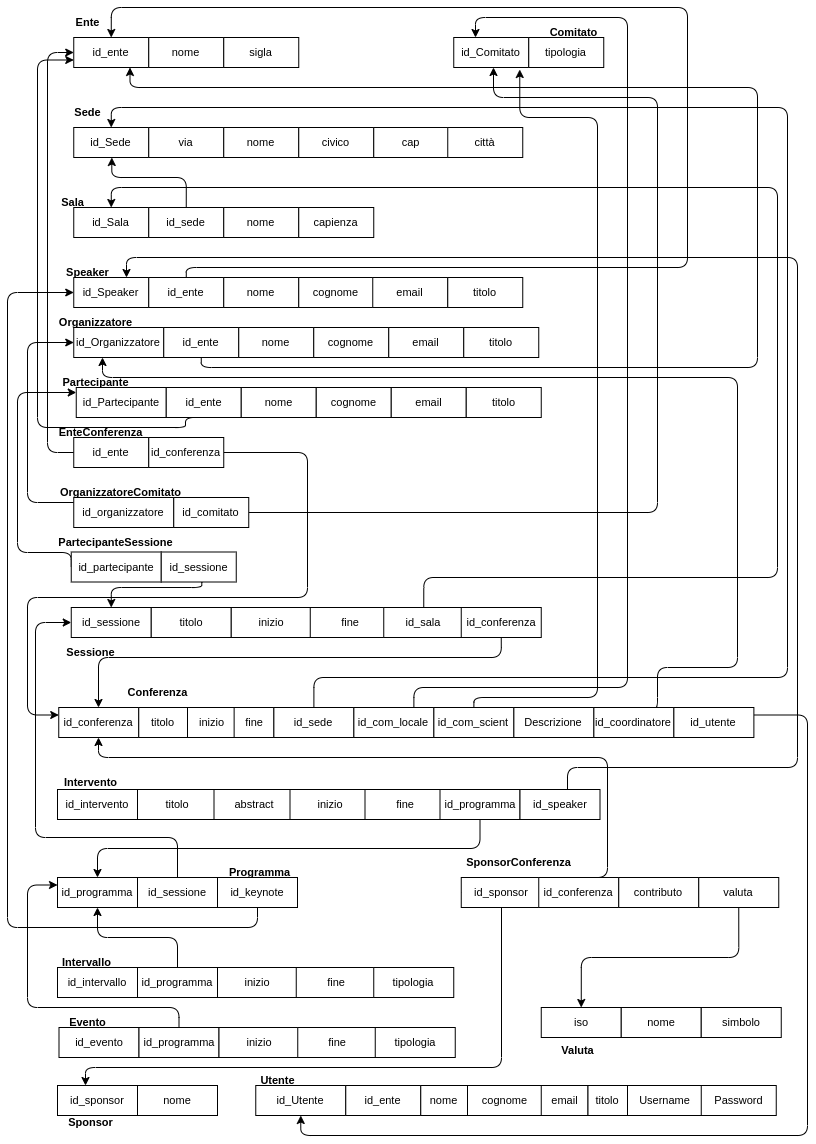
\includegraphics[scale=0.6]{Immagini/Schema_logico.png}\label{fig:schema_logico}
	
\end{figure}